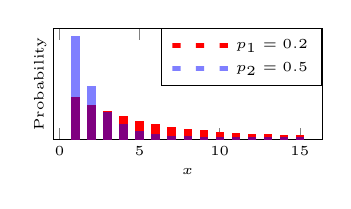
\begin{tikzpicture}
    % \pgfplotsset{ticks = none}
    \tiny
    \begin{axis}[
            xlabel={$x$},
            ylabel={Probability},
            legend style={at={(1,1)},anchor=north east},
            legend style={font=\tiny},
            ymin  = 0,
            ytick = \empty,
            yticklabel=\empty,
            height = 3cm,
            width = 5cm,
            grid style=dashed,
            bar width=1pt,
        ]
        \addplot [
            domain=1:15,
            samples=15,
            color=red,
            ybar,
            draw opacity=1,
            line width = 2pt,
        ]
        {((1-0.2)^(x-1))*0.2};
        \addlegendentry{$p_1=0.2$}

        \addplot [
            domain=1:15,
            samples=15,
            color=blue,
            ybar,
            draw opacity=0.5,
            line width = 2pt,
        ]
        {((1-0.5)^(x-1))*0.5};
        \addlegendentry{$p_2=0.5$}
    \end{axis}
\end{tikzpicture}